\documentclass[a4paper]{article}
\usepackage[italian]{babel}
\usepackage[left=1cm, right=1cm, bottom=2cm, top=2cm]{geometry}
\usepackage{csvsimple}
\usepackage[utf8]{inputenc}
\usepackage{float}
\usepackage{pdfpages}
\usepackage[scaled]{helvet}
\renewcommand\familydefault{\sfdefault} 
\usepackage{pgfplots}
\usepackage{pdflscape}
%opening
\title{Relazione laboratorio Algoritmi Avanzati}
\author{Magarotto Francesco\\Muraro Enrico\\Piva Giulio}

\begin{document}
\begin{titlepage}
  \vspace*{5cm}
  \begin{center}
    \Large\bfseries
    Relazione di laboratorio
  \end{center}
  \begin{center}
    \large
    Corso di Algoritmi Avanzati\\
    Laurea Magistrale in Informatica\\A.A. 2019-2020
  \end{center}
  \vspace{4cm plus 1fill}
  \begin{flushleft}
    \large
    Magarotto Francesco - 1236594\\Muraro Enrico - 1238899 \\Piva Giulio - 1242455
  \end{flushleft}
\end{titlepage}
\newpage


\newpage

%\begin{figure}[H]
%\centering
%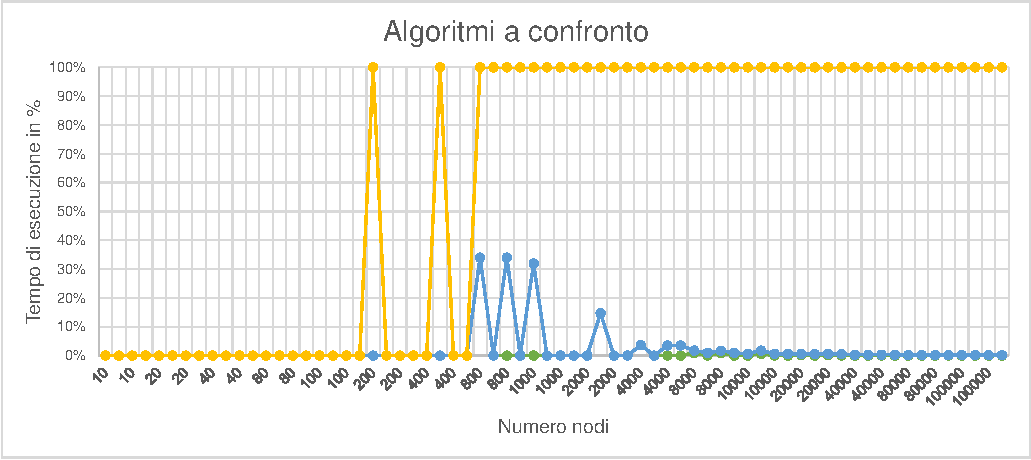
\includegraphics[scale=1]{grafici/confronto.pdf}
%\caption{Grafico che mette in relazione i tempi di esecuzione dei tre algoritmi in base al tempo richiesto per la loro esecuzione}
%\end{figure}
\section{Risultati ottenuti}
\begin{figure}[ht]
	\centering
	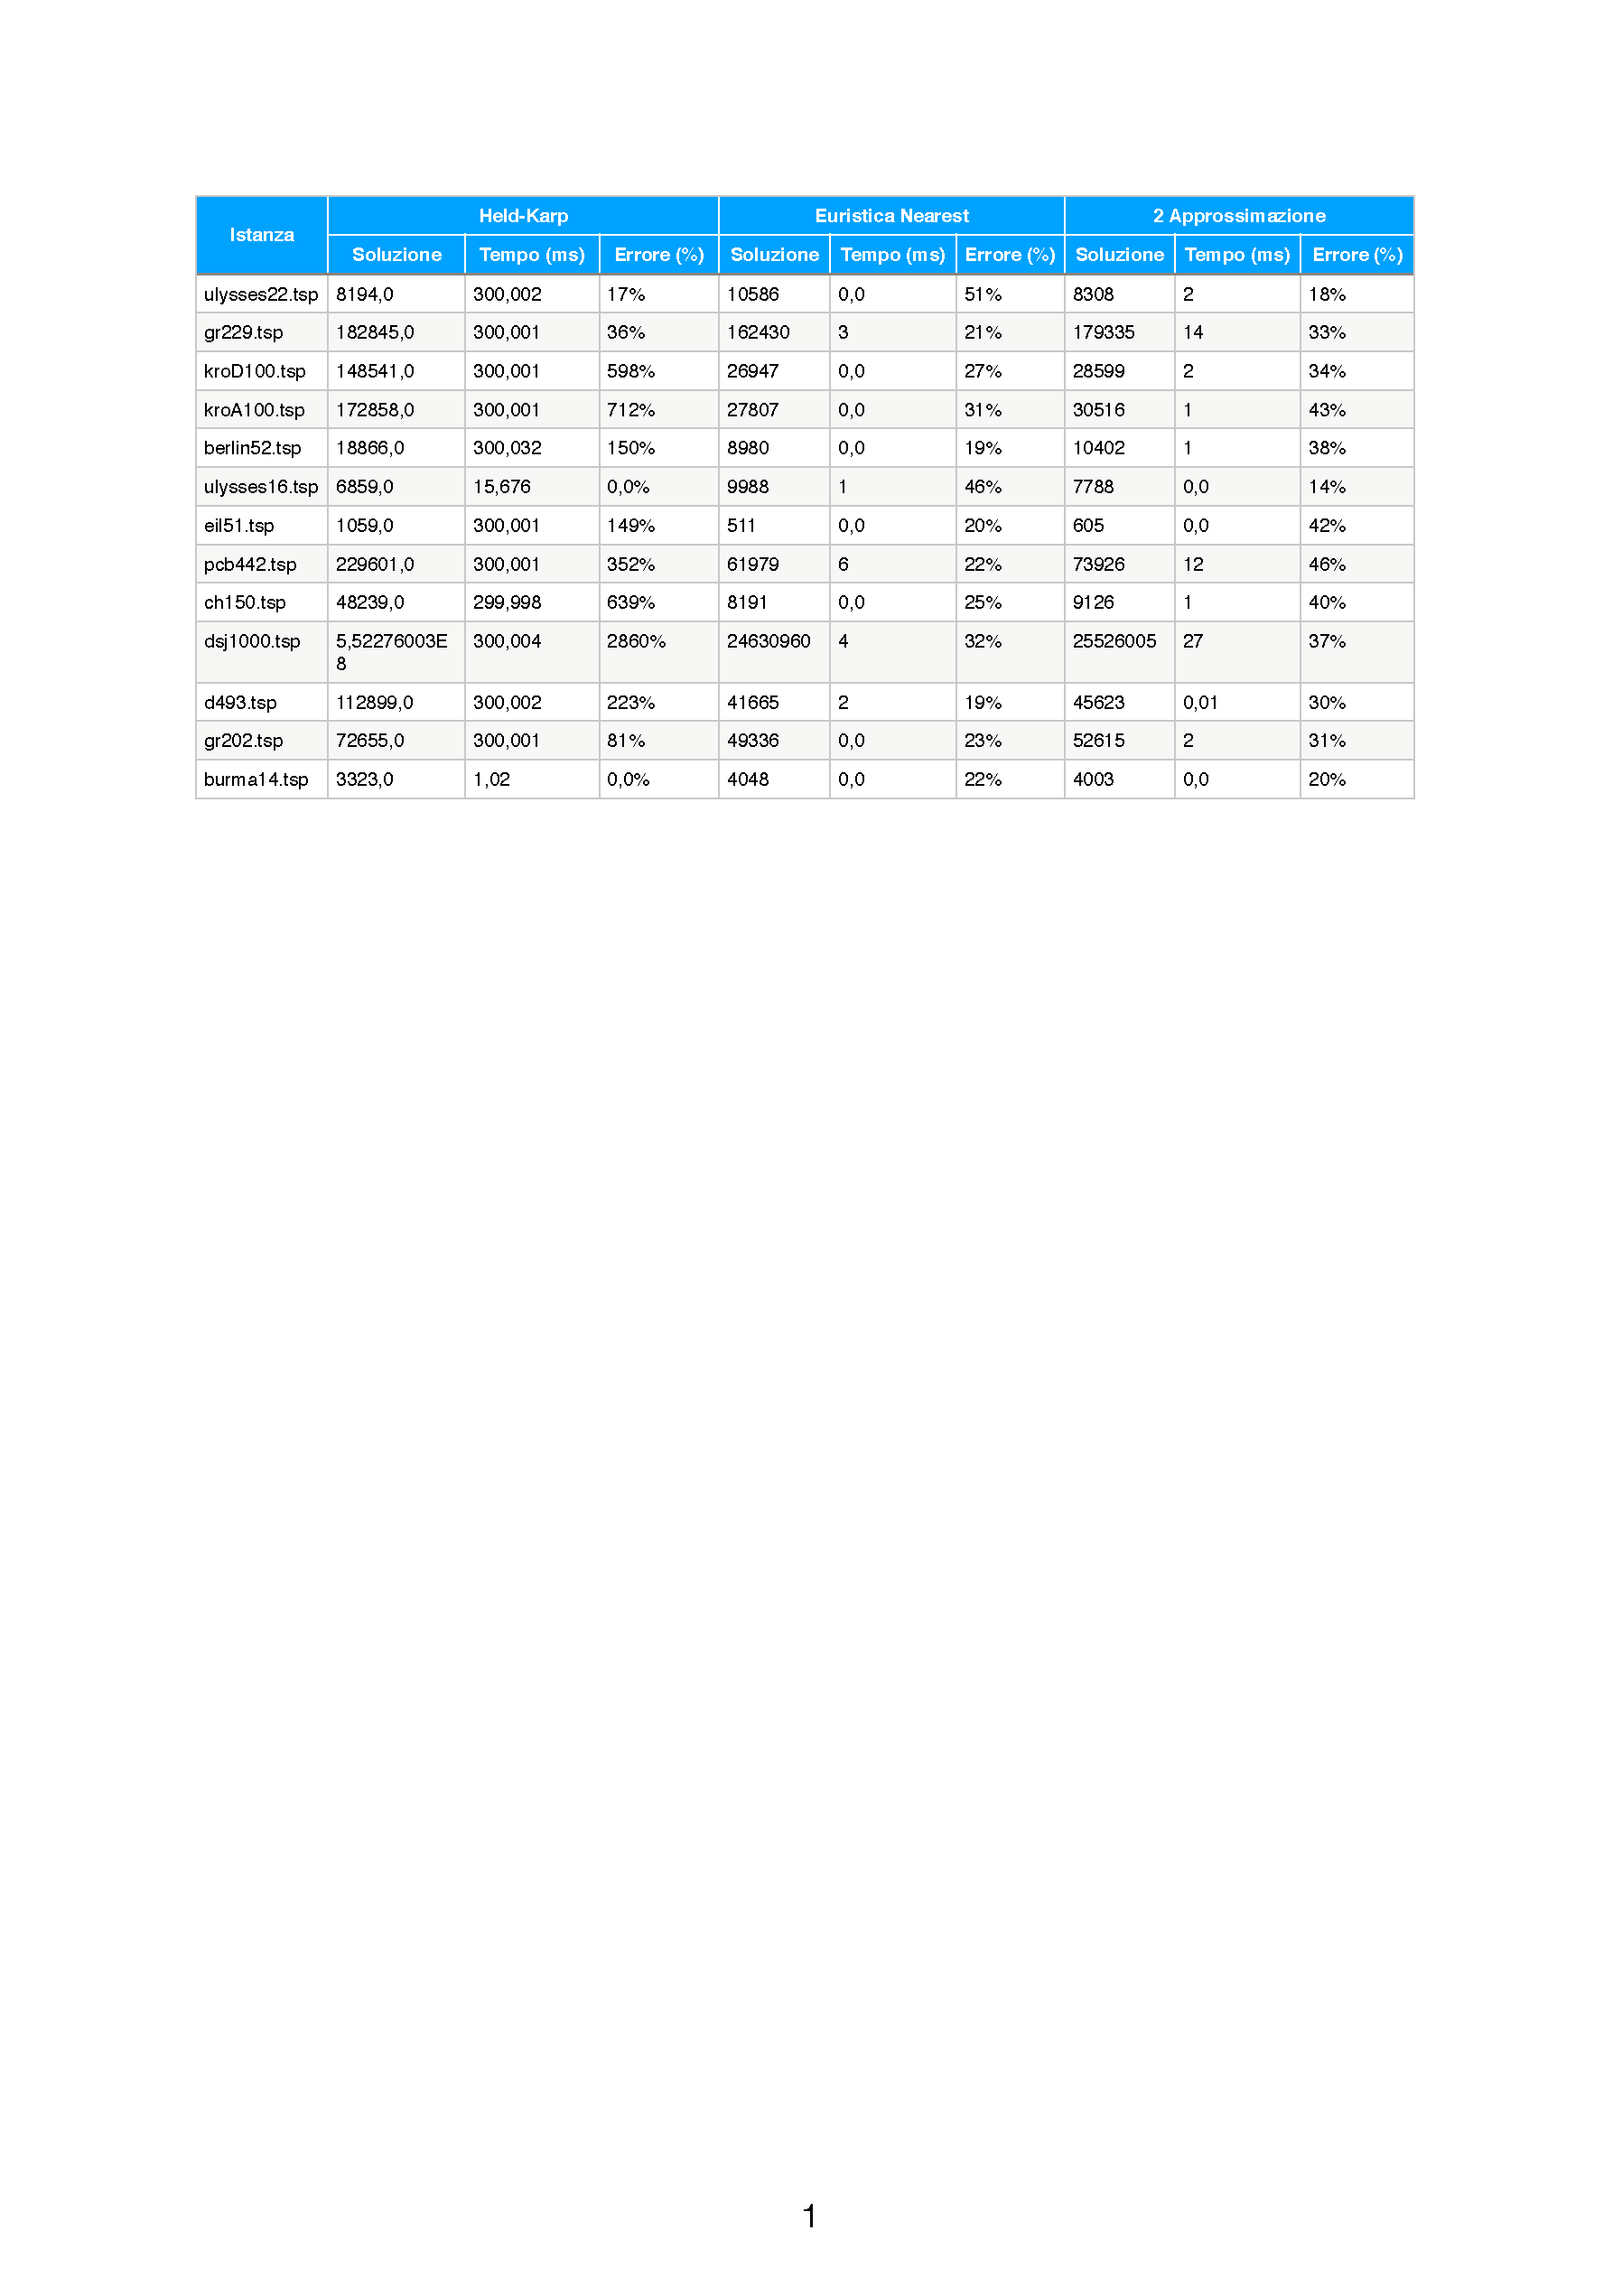
\includepdf[pages=-]{tabellapdf}
\end{figure}
\end{document}
